% Compact PGFPlots panel for sampled qldpc_34_4_5_cap7 BSC correction-class derivative.
% Requires \usepackage{pgfplots} and \pgfplotsset{compat=1.18}.
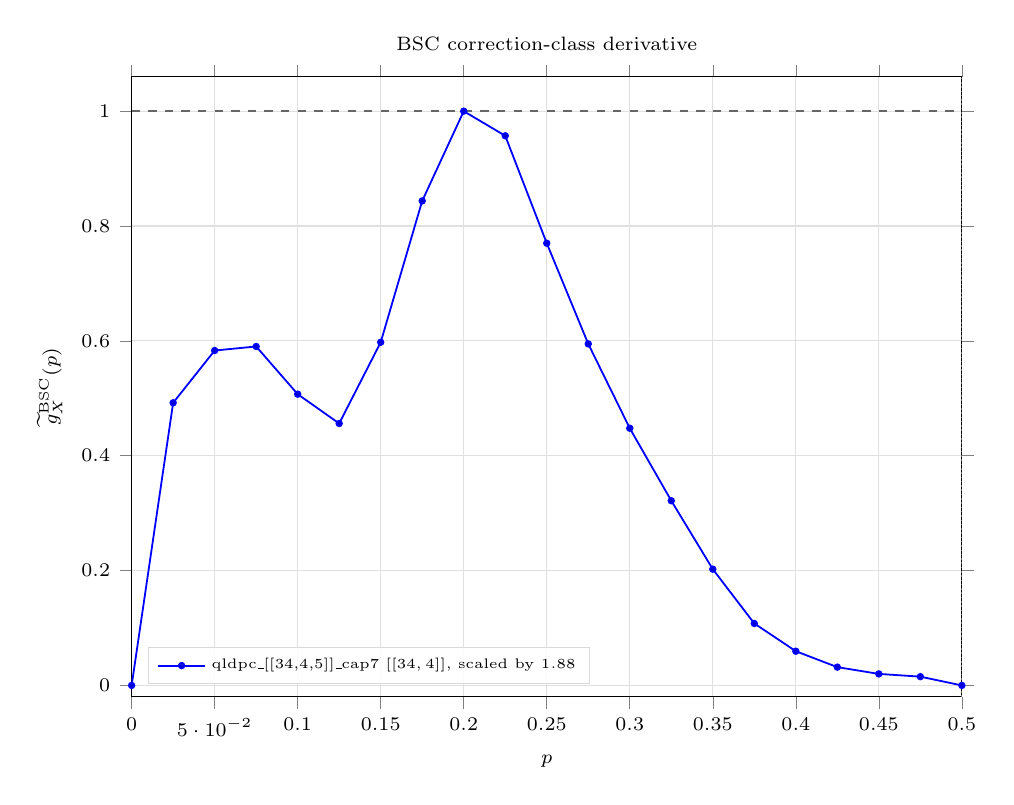
\begin{tikzpicture}
\begin{axis}[
  name=scaledBSCGEXITQldpc3445Cap7Axis,
  width=\linewidth,
  height=0.78\linewidth,
  title={BSC correction-class derivative},
  title style={font=\scriptsize},
  xlabel={$p$},
  ylabel={$\widetilde g_X^{\rm BSC}(p)$},
  xmin=0, xmax=0.5,
  ymin=-0.02, ymax=1.06,
  grid=both,
  major grid style={black!12},
  minor grid style={black!6},
  tick align=outside,
  tick label style={font=\scriptsize},
  label style={font=\scriptsize},
  legend cell align={left},
  legend style={draw=black!15, fill=white, fill opacity=0.82, text opacity=1, at={(0.02,0.02)}, anchor=south west, font=\tiny},
]
\addplot[black!60, densely dotted, line width=0.55pt, forget plot] coordinates {(0.5,-0.02) (0.5,1.06)};
\addplot[black!60, dashed, line width=0.55pt, forget plot] coordinates {(0,1) (0.5,1)};
\addplot+[color=blue, mark=*, mark size=1.0pt, line width=0.65pt]
coordinates {(0,0) (0.025,0.492192072532) (0.05,0.583191782061) (0.075,0.590247701647) (0.1,0.507198562645) (0.125,0.456137632643) (0.15,0.597605132833) (0.175,0.843777787968) (0.2,1) (0.225,0.957127517621) (0.25,0.770049916933) (0.275,0.594716629333) (0.3,0.447810909835) (0.325,0.321635704708) (0.35,0.202448274083) (0.375,0.107853564976) (0.4,0.0595601084857) (0.425,0.0318483630108) (0.45,0.0200653853613) (0.475,0.0152628779013) (0.5,0)};
\addlegendentry{qldpc\_[[34,4,5]]\_cap7 $[[34,4]]$, scaled by $1.88$}
\end{axis}
\end{tikzpicture}
